\section{Selection Sort}
\begin{enumerate}
    \item Prima del passo principale $k$, con $k = 0,\dots, n - 1$, i primi 
    $k$ elementi dell'array sono al loro posto definitivo, cioè sono ordinati
    tra loro e sono minori o uguali degli elementi successivi

    \item Si seleziona l'elemento che andrà collocato in posizione $k$, cioè
    il minimo della parte non ordinata (quindi il minimo tra $A[k],\dots,A[n-1]$)

    \item Lo si colloca in posizione $k$, scambiandolo con l'elemento ivi presente
    \item In questo modo, dopo il passo principale $k$, i primi $k$ elementi
    risultano collocati nella loro posizione definitiva.
\end{enumerate}

\noindent Dopo il passo $n - 2$ la parte non ordinata contiene solo un elemento e, in base
al punto 1, questo è maggiore o uguale dei precedenti, e dunque si trova nella sua
posizione definitiva. Pertanto non è necessario eseguire il passo $n - 1$

\begin{figure}[h]
    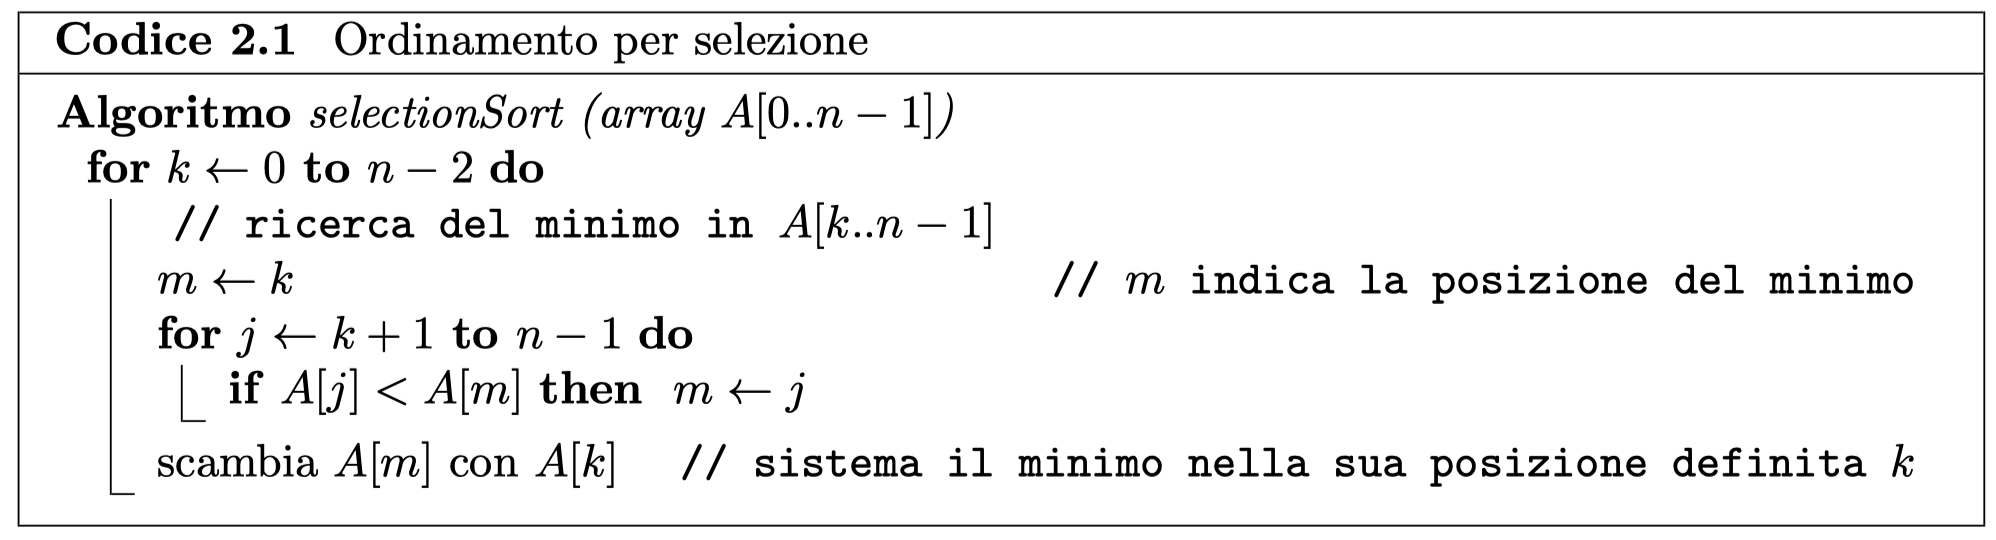
\includegraphics[width=\textwidth]{selectionsort.png}
    \centering
\end{figure}

\subsubsection*{Numero di confronti}
Nell'iterazione $k$ del ciclo principale viene ricercato il minimo della porzione di 
vettore da posizione $k$ a posizione $n - 1$, effettuando quindi $n-k-1$ confronti.
Sommando su tutte le iterazioni $k$ del ciclo principale otteniamo il numero totale
di confronti $\frac{n(n-1)}{2} = \Theta(n^2)$, che vengono eseguiti sempre indipendentemente dal
contenuto dell'array.

\subsubsection*{Spazio}
L'algoritmo, oltre all'array da ordinare, utilizza un numero costante di variabili.
Pertanto la quantità di spazio aggiuntivo è costante.
\clearpage